\documentclass[12pt,a4paper]{article}

% ---------- Core packages for KAIS submission ----------
\usepackage[utf8]{inputenc}
\usepackage[margin=2.5cm]{geometry}
\usepackage{amsmath,amssymb,amsfonts,amsthm}
\usepackage{algorithm}
\usepackage{algpseudocode}
\usepackage{array}
\usepackage{xcolor}
\usepackage{url}
\usepackage{graphicx}
\usepackage{booktabs}
\usepackage{multirow}
\usepackage{tikz}
\usetikzlibrary{positioning,calc,fit,shapes,backgrounds,arrows.meta}
\usepackage{pgfplots}
\pgfplotsset{compat=1.15}
\usepackage{subcaption}
\usepackage{float}
\usepackage{bm}
\usepackage[numbers,sort&compress]{natbib}
\usepackage[hidelinks]{hyperref}
\usepackage[capitalize,noabbrev]{cleveref}

% ---------- Line spacing ----------
\usepackage{setspace}
\onehalfspacing

% ---------- Theorem environments ----------
\theoremstyle{definition}
\newtheorem{theorem}{Theorem}[section]
\newtheorem{lemma}[theorem]{Lemma}
\newtheorem{corollary}[theorem]{Corollary}
\newtheorem{definition}[theorem]{Definition}
\newtheorem{assumption}[theorem]{Assumption}
\newtheorem{remark}[theorem]{Remark}

% ---------- Mathematical operators ----------
\DeclareMathOperator{\ECE}{ECE}
\DeclareMathOperator{\KL}{KL}
\DeclareMathOperator*{\argmax}{arg\,max}
\DeclareMathOperator{\softmax}{softmax}
\newcommand{\E}{\mathbb{E}}
\newcommand{\R}{\mathbb{R}}

\begin{document}

\title{Stochastic PAC-Bayesian Transformers for Network Intrusion Detection and Natural Language Processing Applications}

\author{Roger Nick Anaedevha\thanks{Corresponding author: rogernickanaedevha@gmail.com} \and Alexander G. Trofimov \and Yuri V. Borodachev\\
\small National Research Nuclear University \\ 
\small Moscow Engineering Physics Institute (MEPhI), \\ 
\small Moscow, 115409, Russia}

\date{}
\maketitle

\begin{abstract}
\noindent Transformer architectures dominate contemporary machine learning yet face critical limitations in security applications: vulnerability to adversarial attacks, absence of calibrated uncertainty estimates, and difficulty distinguishing confident predictions from uncertain cases requiring human review. We introduce stochastic Probably Approximately Correct (PAC) Bayesian transformers that convert deterministic attention into probabilistic variants via variational inference, unifying uncertainty quantification and adversarial robustness within a single framework. Our approach replaces fixed attention weights with learned variational distributions and propagates uncertainty through Monte Carlo (MC) sampling, creating moving targets that degrade adversarial effectiveness. We derive joint PAC-Bayesian bounds showing that parameter stochasticity improves both calibration and robustness, with complexity scaling as $\mathcal{O}(\sqrt{\KL(\rho\|\pi)/n})$, where $\KL$ denotes the Kullback-Leibler divergence between the learned posterior $\rho$ and prior $\pi$, and $n$ is the sample size. Across network intrusion detection, toxic content detection, and fake news identification, we achieve $96.8\pm0.8\%$ accuracy with Expected Calibration Error (ECE) of $0.043\pm0.006$, and maintain $88.3\pm1.5\%$ robust accuracy under multiple attack strategies. Uncertainty-guided active learning reduces labeling requirements by 68\%, reaching 95\% of full-data performance with only 35\% of labels.
\end{abstract}

\noindent\textit{Keywords:} adversarial machine learning, transformer architectures, Bayesian neural networks, uncertainty quantification, adversarial robustness, PAC-Bayesian theory

\section{Introduction}

Transformer models excel at capturing long-range dependencies across language, vision, and security applications \citep{vaswani2017attention}. Yet their deterministic computations pose challenges in high-stakes settings where both accuracy and calibrated confidence are essential. Deterministic attention produces fixed decision boundaries that adversaries exploit and yields point predictions without principled uncertainty quantification. In security-critical domains such as network intrusion detection and Natural Language Processing (NLP) applications including toxic content moderation and fake news identification, these shortcomings carry practical consequences: misclassified threats may go undetected, while overconfident predictions provide no signal that human review is warranted.

The adversarial fragility of transformers is well documented. Han et al. \citep{han2021evaluating} demonstrated significant performance degradation under crafted perturbations in network intrusion detection systems. Canonical attacks including the Fast Gradient Sign Method (FGSM) \citep{goodfellow2014explaining}, Projected Gradient Descent (PGD) \citep{madry2018towards}, and Carlini-Wagner (C\&W) optimization \citep{carlini2017towards} remain consistently effective. Furthermore, functionality-preserving attacks pose significant concerns in cybersecurity \citep{mccarthy2022functionality}, where attackers maintain operational characteristics while evading detection. Post-hoc calibration methods often fail under distribution shift or adversarial attack \citep{guo2017calibration,desai2020calibration}, limiting practical deployment reliability.

Distribution shift presents a pervasive challenge in security applications. Network traffic patterns evolve as attackers develop new strategies, the language used in toxic content shifts with cultural trends, and misinformation tactics adapt over time. These non-stationary conditions mean that models trained on one distribution must generalize to shifted or entirely novel distributions at deployment. Out-of-Distribution (OOD) generalization has received growing attention, with recent work demonstrating that transformer architectures can achieve zero-shot inference on systems fundamentally different from those seen during training \citep{zhai2025bridging}. However, most existing approaches address OOD generalization without jointly considering adversarial robustness and calibrated uncertainty, which are equally essential for trustworthy deployment.

The PAC-Bayesian framework, rooted in the Probably Approximately Correct learning theory introduced by Valiant \citep{valiant1984theory} and extended to stochastic predictors by McAllester \citep{mcallester1998some,mcallester2003pac}, provides a natural theoretical foundation for addressing these challenges. PAC-Bayesian bounds relate the generalization error of a stochastic classifier to the Kullback-Leibler (KL) divergence between a data-dependent posterior and a data-independent prior, offering tighter and more computable complexity measures than classical Vapnik-Chervonenkis dimension arguments.

We address the shortcomings of deterministic transformers by introducing stochastic PAC-Bayesian transformers that perform three key operations. First, we apply variational inference to attention projections and embeddings to model parameter uncertainty explicitly. Second, we propagate uncertainty through MC sampling during both training and inference. Third, we incorporate Expectation-over-Transformations (EOT) adversarial training with a multi-objective loss balancing accuracy, calibration, robustness, and complexity via the KL divergence term $\KL(\rho\|\pi)$ between the learned posterior $\rho$ and prior $\pi$. Our theoretical framework establishes joint bounds linking empirical calibration and robustness to posterior complexity and controlled stochasticity.

\subsection{Contributions}

This work makes four principal contributions. First, we introduce an architecture where Bayesian attention and variational embeddings transform deterministic modules into probabilistic ones while remaining computationally tractable via the reparameterization trick and head-wise sampling strategies. Second, we develop a unified training objective combining predictive loss, calibration surrogate, adversarial loss under EOT, and PAC-Bayesian complexity regularization into a single differentiable objective. Third, we formulate joint PAC-Bayesian bounds guaranteeing both calibration and robustness with convergence rates depending on the KL divergence between posterior and prior distributions and the sample size. Fourth, we demonstrate practical effectiveness across network intrusion detection and NLP, achieving 96.8\% accuracy, ECE of 0.043, and 88.3\% retention under multiple attacks, while active learning reduces labeling by 68\%.

\section{Problem Formulation}

\subsection{Multi-Domain Security Framework}

We formulate a domain-agnostic problem encompassing security-critical classification across both continuous (tabular) and discrete (textual) data. Let $\mathcal{D}=\{d_{1},\dots,d_{K}\}$ denote a finite set of $K$ domains, where each domain $d_i$ is characterized by an input space $\mathcal{X}_{d_i}$, a label space $\mathcal{Y}_{d_i}$, a data distribution $P_{d_i}(X,Y)$, and an adversary class $\mathcal{A}_{d_i}$ defining permissible perturbations. Our goal is to learn a single stochastic transformer $f_{\phi}$ handling heterogeneous inputs and producing calibrated predictions across all domains. The model maps an input $x\in\mathcal{X}_{d}$ to a predictive distribution over labels in $\mathcal{Y}_d$ with uncertainty estimates:
\begin{equation}
f_{\phi}(x) \in \Delta^{|\mathcal{Y}_{d}|-1} \times \mathbb{R}_{+} \times \mathbb{R}_{+},\quad \forall d\in\mathcal{D}
\end{equation}
where $\Delta^{|\mathcal{Y}_{d}|-1}$ denotes the $(|\mathcal{Y}_{d}|-1)$-dimensional probability simplex (the set of non-negative vectors summing to one), $\mathbb{R}_{+}$ represents non-negative reals used for epistemic and aleatoric uncertainty scores, and $\phi$ parameterizes the variational posteriors over model weights.

To simultaneously achieve predictive accuracy, calibrated uncertainty, and adversarial robustness, we pose the constrained optimization:
\begin{equation}
\label{eq:unified_objective}
\min_{\phi}\;\;\mathbb{E}_{d\sim\mathcal{D}}\Big[\mathcal{L}_{\mathrm{pred}}(f_{\phi},P_{d}) + \alpha\,\mathcal{L}_{\mathrm{cal}}(f_{\phi},P_{d}) + \beta\,\mathcal{L}_{\mathrm{rob}}(f_{\phi},\mathcal{A}_{d})\Big]
\end{equation}
subject to domain-specific constraints on ECE, defined as $\ECE_{d}(f_{\phi}) \le \delta_{d}$. Here $\mathcal{L}_{\mathrm{pred}}$ measures classification accuracy via the cross-entropy loss, $\mathcal{L}_{\mathrm{cal}}$ is a calibration surrogate computed as the Brier score, $\mathcal{L}_{\mathrm{rob}}$ measures adversarial loss under attack class $\mathcal{A}_{d}$, and $\alpha, \beta > 0$ are trade-off coefficients.

\subsection{Unified Architecture and Threat Model}

We employ a single transformer backbone with domain-shared parameters across all layers except input and output projections. Domain-specific nuances (tokenization for text, normalization for tabular data) are handled via the input embedding layer $\phi_d: \mathcal{X}_d \to \mathbb{R}^{d_{\text{emb}}}$, where $d_{\text{emb}}$ denotes the embedding dimensionality. All attention blocks operate on $\mathbb{R}^{d_{\text{emb}}}$ and share parameters across domains, enabling transfer learning.

For tabular intrusion detection, we adopt $\ell_\infty$-bounded perturbations with protocol constraints ensuring perturbed samples remain valid network traffic. For textual inputs, adversaries employ token-level substitutions using semantically similar words, character-level perturbations, and paraphrase-based transformations, all subject to semantic similarity constraints via sentence embeddings and fluency constraints via language model perplexity. Detailed threat model specifications, including parametric adversary definitions $\mathcal{A}_d(\epsilon, \tau, \rho, \mathcal{C}_d)$ with perturbation budget $\epsilon$, temporal coherence constraint $\tau$, poisoning rate $\rho$, and domain constraints $\mathcal{C}_d$, are provided in Appendix~A.

\section{Related Work}

Transformers underpin state-of-the-art performance across NLP and vision \citep{vaswani2017attention,devlin2019bert,dosovitskiy2021image}, but their adversarial fragility is well documented \citep{kheddar2024transformers,xu2024large}. The TextAttack framework \citep{morris2020textattack} unifies attack methods including TextFooler \citep{jin2020bert} and BERT-Attack \citep{li2020bert}. Certified defenses like SAFER \citep{ye2020safer} offer probabilistic guarantees but struggle to scale. Recent work on transformer-based OOD generalization includes Zhai et al. \citep{zhai2025bridging}, who demonstrated zero-shot inference on unseen dynamical systems using a hybrid transformer-reservoir computing framework, illustrating both the promise and limitations of transformers under distribution shift.

Bayesian neural networks model parameter uncertainty \citep{abdar2021review}, with methods including MC-Dropout \citep{gal2016dropout} and variational inference \citep{blundell2015weight}. Stochastic attention variants like Sinkformers \citep{sander2023sinkformers} and BayesFormer \citep{sankararaman2022bayesformer} improve generalization but lack explicit robustness analysis. Our design differs from BayesFormer in four respects. First, BayesFormer derives principled dropout placement from variational inference, applying separate masks to key, query, and value vectors without introducing new parameters; our method replaces the projection matrices with learned Gaussian distributions, providing per-parameter variance that adapts to data evidence. Second, our variational embeddings propagate input-level uncertainty through the network, which BayesFormer does not address. Third, BayesFormer explicitly acknowledges that adversarial robustness remains unexplored in their framework; our method integrates EOT adversarial training directly into the variational objective. Fourth, we provide joint PAC-Bayesian bounds (Theorem~\ref{thm:joint_bound}) connecting calibration and robustness through the KL divergence, which BayesFormer lacks. Extended related work appears in Appendix~B.

Specialized transformer robustness methods have advanced along several complementary directions. Shi et al. \citep{shi2020robustness} introduced the first formal verification algorithm for self-attention, and RanMASK \citep{zeng2023ranmask} provides certified text robustness via randomized masking. Architecture-specific adversarial training strategies for vision transformers reveal that gradient masking during training improves robustness \citep{mo2022adversarial}, while Jain et al. \citep{jain2024towards} identified floating-point underflow in attention as a source of gradient masking and proposed Adaptive Attention Scaling. Efficient robust fine-tuning via low-rank adapters (FullLoRA-AT, \citealt{yuan2024fulllora}) achieves adversarial robustness with approximately five percent of learnable parameters. Our work is complementary to these architecture-specific methods: we provide a unified theoretical framework connecting calibration and robustness through PAC-Bayesian bounds, and our EOT training can be combined with the architectural insights from these specialized approaches.

\section{Methodology}

\subsection{Stochastic Transformer Architecture}

\begin{figure}[!t]
\centering
\includegraphics[width=0.75\columnwidth]{Paper2_revised_v1/architecture_v20a.png}
\caption{Stochastic PAC-Bayesian transformer architecture. Clean and adversarial inputs pass through variational embeddings into a transformer with Bayesian attention at selected layers. MC sampling propagates uncertainty. Training minimizes multi-objective loss combining accuracy, calibration, robustness, and PAC-Bayesian KL regularization.}
\label{fig:architecture}
\end{figure}

\subsubsection{Bayesian Attention Mechanism}

Traditional deterministic attention computes:
\begin{equation}
\text{Attn}(\bm{Q}, \bm{K}, \bm{V}) = \softmax\left(\frac{\bm{Q}\bm{K}^\top}{\sqrt{d_k}}\right)\bm{V}
\end{equation}
where $\bm{Q} = \bm{X}\bm{W}_Q$, $\bm{K} = \bm{X}\bm{W}_K$, $\bm{V} = \bm{X}\bm{W}_V$ are query, key, and value matrices obtained by multiplying the input $\bm{X} \in \mathbb{R}^{n \times d}$ (with $n$ denoting sequence length and $d$ the model dimension) by fixed projection matrices $\bm{W}_Q, \bm{W}_K, \bm{W}_V \in \mathbb{R}^{d \times d_k}$, and $d_k$ is the key dimensionality.

We replace fixed projections with stochastic weights sampled from learned distributions:
\begin{equation}
\label{eq:bayes_att}
\text{BayesAttn}(\bm{Q}, \bm{K}, \bm{V}) = \mathbb{E}_{\bm{W}_Q, \bm{W}_K, \bm{W}_V \sim q_\phi}\Big[\softmax\Big(\frac{(\bm{X}\bm{W}_Q)(\bm{X}\bm{W}_K)^\top}{\sqrt{d_k}}\Big)(\bm{X}\bm{W}_V)\Big]
\end{equation}
where $q_\phi$ denotes the variational posterior over projection weights parameterized by $\phi$. Implementation uses the reparameterization trick: each weight is expressed as $\bm{W}=\bm{\mu}+\bm{\sigma}\odot\bm{\epsilon}$, where $\bm{\mu}$ and $\bm{\sigma}$ are learned mean and standard deviation parameters, $\bm{\epsilon}\sim\mathcal{N}(\bm{0},\bm{I})$ is standard Gaussian noise, and $\odot$ denotes elementwise multiplication. This enables unbiased gradient estimation through the variational parameters. We perform head-wise sampling where each attention head draws independent weight samples for computational tractability.

\begin{remark}[Distinction from BayesFormer]
Unlike BayesFormer, which re-positions existing dropout masks without adding parameters, our method introduces explicit mean $\bm{\mu}$ and log-variance $\log\bm{\sigma}^2$ for every projection weight, approximately doubling the parameter count of Bayesian layers but enabling per-parameter posterior adaptation. The variance of each weight reflects the data-driven uncertainty about that parameter, providing richer uncertainty information than a global dropout rate.
\end{remark}

This design provides three benefits: automatic uncertainty calibration via learned posterior distributions $q_\phi(\bm{W})$ without domain-specific tuning, a moving-target defense where adversaries must succeed across multiple stochastic model instantiations, and regularization through $\KL(q_\phi\|\pi)$ preventing overfitting. Variational embeddings represent inputs as Gaussian variables: $z=\bm{\mu}_{\text{emb}}(x)+\bm{\sigma}_{\text{emb}}(x)\odot\bm{\epsilon}$ where $\bm{\epsilon}\sim\mathcal{N}(\bm{0},\bm{I})$, propagating input ambiguity through network layers. Detailed analysis of cross-domain robustness properties appears in Appendix~C.

\begin{algorithm}[t]
\caption{Bayesian Attention with Uncertainty Propagation}
\label{alg:bayesian_attention}
\begin{algorithmic}[1]
\Require Input $X\in\mathbb{R}^{n\times d}$; variational parameters $\{\mu_{W_Q},\sigma_{W_Q}\}$, $\{\mu_{W_K},\sigma_{W_K}\}$, $\{\mu_{W_V},\sigma_{W_V}\}$; MC samples $S$
\Ensure Output $Y\in\mathbb{R}^{n\times d}$; epistemic uncertainty $U_{\text{epi}}$; KL term $\mathcal{L}_{\mathrm{KL}}$
\For{$s=1$ to $S$}
  \State Sample noise $\epsilon_Q,\epsilon_K,\epsilon_V\sim\mathcal{N}(0,I)$
  \State Compute $W_Q^{(s)}\gets \mu_{W_Q}+\sigma_{W_Q}\odot\epsilon_Q$ (similarly for $W_K, W_V$)
  \State Project: $Q^{(s)}\gets XW_Q^{(s)}$, $K^{(s)}\gets XW_K^{(s)}$, $V^{(s)}\gets XW_V^{(s)}$
  \State Compute attention: $A^{(s)}\gets \softmax(Q^{(s)}{K^{(s)}}^\top/\sqrt{d_k})$
  \State Compute output: $Y^{(s)}\gets A^{(s)}V^{(s)}$
\EndFor
\State Compute mean: $Y\gets \frac{1}{S}\sum_s Y^{(s)}$, $\bar{A}\gets \frac{1}{S}\sum_s A^{(s)}$
\State Compute uncertainty: $U_{\text{epi}}\gets \frac{1}{n^2}\sum_{i,j}\text{Var}[A^{(s)}_{ij}]$
\State Compute KL: $\mathcal{L}_{\mathrm{KL}}\gets \tfrac{1}{2}\sum_{w\in\{Q,K,V\},j} (\mu_{w,j}^2+\sigma_{w,j}^2-1-\log\sigma_{w,j}^2)$
\State \Return $Y,\,U_{\text{epi}},\,\mathcal{L}_{\mathrm{KL}}$
\end{algorithmic}
\end{algorithm}

\subsection{Training with Expectation-Over-Transformations}

We train with EOT so adversaries must defeat the expected stochastic model. Adversarial examples are generated by solving:
\begin{equation}
\label{eq:eot}
x^{\text{adv}}
\in
\arg\max_{x'\in\mathcal{A}_\epsilon(x)}\;
\mathbb{E}_{\theta\sim q_\phi}[\mathcal{L}(f_\theta(x'),y)]
\end{equation}
where $\mathcal{A}_\epsilon(x)$ is the set of permissible perturbations of $x$ within budget $\epsilon$, $q_\phi$ is the variational posterior, $f_\theta$ is the model parameterized by a sample $\theta$ from $q_\phi$, $\mathcal{L}$ is the classification loss, and $y$ is the true label.

The total loss balances accuracy, calibration, robustness, and complexity:
\begin{equation}
\label{eq:total_loss}
\mathcal{L}_{\text{tot}}
=
\mathcal{L}_{\text{cls}}
+\lambda_{1}\,\mathcal{L}_{\mathrm{KL}}
+\lambda_{2}\,\mathcal{L}_{\text{cal}}
+\lambda_{3}\,\mathcal{L}_{\text{adv}}
+\lambda_{4}\,\mathcal{L}_{\text{reg}}
\end{equation}
where $\mathcal{L}_{\text{cls}}=-\mathbb{E}[\log p_\theta(y|x)]$ is the classification cross-entropy, $\mathcal{L}_{\mathrm{KL}}=\sum_l \KL(q_\phi(\theta_l)\| p(\theta_l))$ is the PAC-Bayesian complexity penalty summed over layers $l$, $\mathcal{L}_{\text{cal}}$ is the Brier score calibration surrogate, $\mathcal{L}_{\text{adv}}$ is the EOT adversarial loss computed over perturbed inputs, and $\mathcal{L}_{\text{reg}}$ is an $\ell_2$ weight decay term. The coefficients $\lambda_1, \lambda_2, \lambda_3, \lambda_4 > 0$ control the relative importance of each objective. Complete training algorithm appears in Appendix~D.

\subsection{Theoretical Analysis}

\begin{assumption}[Regularity Conditions]
\label{assump:regularity}
We assume: (i) the calibration loss $\ell_{\text{cal}}$ and robust loss $\ell_{\text{rob}}$ are bounded in the interval $[0,1]$; (ii) the stochastic transformer $f_\theta$ is $L$-Lipschitz continuous in its parameters $\theta$, meaning $\|f_{\theta_1}(x) - f_{\theta_2}(x)\| \leq L \|\theta_1 - \theta_2\|$ for all inputs $x$; (iii) the KL divergence $\KL(q_\phi(\theta) \| \pi(\theta))$ between the variational posterior $q_\phi$ and prior $\pi$ is finite; and (iv) the parameters satisfy $\|\theta\|_2 \le B$ almost surely under both $q_\phi$ and prior $\pi$, where $B > 0$ is a known bound.
\end{assumption}

\begin{theorem}[Joint Calibration and Robustness Bound]
\label{thm:joint_bound}
Under Assumption~\ref{assump:regularity}, let $\pi$ be a prior distribution over stochastic transformers fixed before observing data, and let $\rho$ be the learned posterior given a training sample $S$ of size $n$ drawn independently from the data distribution. For any confidence level $\delta \in (0,1)$, the following bounds hold simultaneously with probability at least $1-\delta$ over the random draw of $S$:
\begin{equation}
\label{eq:calibration_bound}
\mathbb{E}_{h\sim\rho}[\ECE(h)]
\;\le\;\mathbb{E}_{h\sim\rho}[\widehat{\ECE}_S(h)]
+\sqrt{\frac{2(\KL(\rho\|\pi)+\log\frac{4\sqrt{n}}{\delta})}{n}}
\end{equation}
\begin{equation}
\label{eq:robustness_bound}
\mathbb{E}_{h\sim\rho}[\text{RobustLoss}_\epsilon(h)]
\;\le\;\mathbb{E}_{h\sim\rho}[\widehat{\text{RobustLoss}}_{\epsilon,S}(h)]
+\sqrt{\frac{2(\KL(\rho\|\pi)+\log\frac{4\sqrt{n}}{\delta})}{n}}
+\mathcal{R}_\epsilon(\sigma^2)
\end{equation}
where $\widehat{\ECE}_S(h)$ and $\widehat{\text{RobustLoss}}_{\epsilon,S}(h)$ are the empirical calibration error and robust loss on $S$, and $\mathcal{R}_\epsilon(\sigma^2) = \beta \exp(-\epsilon^2/(2\sigma^2))$ is a stochasticity bonus term with $\beta = L^2 B^2$ and $\sigma^2$ denoting the posterior variance.
\end{theorem}

The calibration bound follows standard PAC-Bayesian complexity control via $\KL(\rho\|\pi)$. The robustness bound includes the stochasticity bonus $\mathcal{R}_\epsilon(\sigma^2)$ decaying exponentially in $\epsilon^2/\sigma^2$, formalizing how parameter variance attenuates adversarial effectiveness. Complete proofs appear in Appendix~E.

\begin{corollary}[Optimal Stochasticity]
\label{cor:optimal_stochasticity}
Balancing calibration and robustness objectives yields an optimal posterior variance:
\begin{equation}
\sigma^*\;=\;\sqrt{\frac{\epsilon^2}{\log(\beta\sqrt{n}/\lambda_{\text{cal}})}}
\end{equation}
where $\lambda_{\text{cal}}$ is the relative calibration weight. Optimal variance increases with perturbation budget $\epsilon$ and decreases logarithmically with sample size $n$.
\end{corollary}

\section{Experimental Evaluation}

\subsection{Datasets, Setup, and Hyperparameter Selection}

We evaluate across three domains using nine datasets summarized in Table~\ref{tab:datasets}. Network intrusion detection uses CIC-IoT-2023 \citep{neto2023ciciot2023}, CSE-CICIDS2018 \citep{sharafaldin2018toward}, and UNSW-NB15 \citep{moustafa2015unsw}. Toxic content detection uses MetaHate \citep{kirk2024metahate} including HatEval \citep{basile2019semeval} and Founta \citep{founta2018large} subsets. Fake news detection uses LIAR \citep{wang2017liar}, FakeNewsNet \citep{shu2020fakenewsnet}, and ISOT \citep{ahmed2018detecting}. Detailed preprocessing pipelines appear in Appendix~F.

\begin{table}[t]
\caption{Dataset Summary}
\label{tab:datasets}
\centering
\small
\setlength{\tabcolsep}{3pt}
\begin{tabular}{@{}llrrl@{}}
\toprule
Domain & Dataset & Samples & Features/Tokens & Classes\\
\midrule
Network & CIC-IoT-2023 & 697K & 40 features & 8 \\
Network & CSE-CICIDS2018 & 2.2M & 79 features & 14 \\
Network & UNSW-NB15 & 211K & 44 features & 2 \\
Toxic & MetaHate & 1.2M & 512 tokens & 2--4 \\
Toxic & HatEval & 13K & 512 tokens & 2 \\
Toxic & Founta & 80K & 512 tokens & 4 \\
Fake News & LIAR & 12.8K & 256 tokens & 6 \\
Fake News & FakeNewsNet & 23.2K & 512 tokens & 2 \\
Fake News & ISOT & 44.9K & 512 tokens & 2 \\
\bottomrule
\end{tabular}
\end{table}

We employ 5-fold stratified cross-validation with leakage control: author/outlet disjointness for MetaHate/FakeNewsNet, speaker consistency for LIAR, and timestamp ordering for network datasets. We compare against Deterministic BERT \citep{devlin2019bert}, MC-Dropout \citep{gal2016dropout}, Temperature Scaling \citep{guo2017calibration}, Deep Ensembles \citep{lakshminarayanan2017simple}, and BayesFormers \citep{sankararaman2022bayesformer}. We use the AdamW optimizer \citep{loshchilov2019decoupled} with learning rate $2\times 10^{-5}$, batch size 32 with gradient accumulation to effective batch size 128, weight decay $10^{-2}$, and cosine learning rate scheduling with linear warmup over 10\% of training steps.

Loss weights were selected via a two-stage grid search. In the first stage, we searched over $\lambda_1 \in \{0.001, 0.005, 0.01, 0.05\}$, $\lambda_2 \in \{0.01, 0.05, 0.1\}$, $\lambda_3 \in \{0.1, 0.2, 0.5\}$, and $\lambda_4 \in \{0.0005, 0.001, 0.005\}$ using a 20\% validation split on one representative dataset per domain (CIC-IoT-2023, MetaHate, LIAR). In the second stage, we selected the configuration maximizing a composite score of validation accuracy plus $(1-\text{ECE})$ minus robust loss. The selected values ($\lambda_1{=}0.01$, $\lambda_2{=}0.05$, $\lambda_3{=}0.2$, $\lambda_4{=}0.001$) were then fixed across all datasets. Bayesian layer placement at layers 3, 6, 9, and 12 was determined by the ablation in Appendix~H (Table~H.3). All baselines use the same preprocessing, splits, and evaluation protocol; baseline-specific hyperparameters follow their original papers. Complete configuration appears in Appendix~F.

\subsection{Main Results}

\begin{table}[t]
\caption{Overall Performance Across All Domains}
\label{tab:overall}
\centering
\small
\setlength{\tabcolsep}{4pt}
\begin{tabular}{@{}lccccc@{}}
\toprule
Domain & Acc. & F1 & ECE & Datasets\\
\midrule
Network Intrusion & $96.8 \pm 0.7$ & $96.5 \pm 0.8$ & $0.042 \pm 0.005$ & 3 \\
Toxic Content     & $96.2 \pm 0.9$ & $95.8 \pm 1.0$ & $0.049 \pm 0.007$ & 3 \\
Fake News         & $97.1 \pm 0.7$ & $96.8 \pm 0.8$ & $0.037 \pm 0.006$ & 3 \\
\midrule
Average  & $96.8 \pm 0.8$ & $96.4 \pm 0.9$ & $0.043 \pm 0.006$ & 9 \\
\bottomrule
\end{tabular}
\end{table}

Statistical significance was assessed using paired $t$-tests with Bonferroni correction ($\alpha = 0.05/n_{\text{comparisons}}$); all reported improvements are significant ($p < 0.001$). Table~\ref{tab:overall} summarizes performance across domains. Our framework achieves 96.8$\pm$0.8\% accuracy with ECE of 0.043$\pm$0.006, consistently outperforming all baselines. Per-dataset breakdown appears in Appendix~G.

\begin{table}[!t]
\caption{Adversarial Robustness (Average Across Datasets)}
\label{tab:adv_robust}
\centering
\small
\begin{tabular}{@{}lccccc@{}}
\toprule
Method & Clean & FGSM & PGD & C\&W & Retention \\
\midrule
Deterministic BERT & 86.4 & 44.1 & 40.5 & 37.3 & 47.7\% \\
MC-Dropout & 87.1 & 52.3 & 48.7 & 45.2 & 60.1\% \\
Deep Ensembles & 89.2 & 61.4 & 58.1 & 54.6 & 68.8\% \\
Our Method & 96.2 & 86.7 & 83.8 & 81.1 & 88.3\% \\
\bottomrule
\end{tabular}
\end{table}

Table~\ref{tab:adv_robust} shows adversarial robustness. Our method achieves 88.3$\pm$1.5\% average retention across FGSM, PGD, C\&W, and TextFooler attacks, compared to 47.7\% for Deterministic BERT, 60.1\% for MC-Dropout, and 68.8\% for Deep Ensembles.

\begin{table}[!t]
\caption{Controlled Comparison: All Methods with PGD Adversarial Training}
\label{tab:controlled_adv}
\centering
\small
\begin{tabular}{@{}lcccc@{}}
\toprule
Method & Clean & PGD & Retention & $\Delta$ vs Ours \\
\midrule
Det. BERT + AdvTrain & 88.7 & 64.1 & 72.3\% & $-$16.0 \\
MC-Dropout + AdvTrain & 89.4 & 68.6 & 76.8\% & $-$11.5 \\
Ensembles + AdvTrain  & 90.1 & 71.5 & 79.4\% & $-$8.9 \\
BayesFormers + AdvTrain & 90.8 & 73.2 & 80.6\% & $-$7.7 \\
Our Method (full) & 96.2 & 83.8 & 88.3\% & --- \\
\bottomrule
\end{tabular}
\end{table}

To address the concern that robustness gains may stem primarily from adversarial training rather than Bayesian attention, Table~\ref{tab:controlled_adv} presents a controlled comparison where all methods receive the same PGD adversarial training (10 steps, budget $\epsilon=0.1$). Under this controlled setting, Deterministic BERT with adversarial training achieves 72.3\% retention, MC-Dropout achieves 76.8\%, Deep Ensembles achieve 79.4\%, and BayesFormers achieve 80.6\%. Our method maintains an 8.9 percentage point advantage over the strongest adversarially-trained baseline, confirming that Bayesian attention contributes meaningful robustness beyond what adversarial training alone provides. Furthermore, our ablation (Table~\ref{tab:ablation}) shows that removing adversarial training from our method reduces retention to 70.0\%, which still exceeds deterministic baselines, demonstrating the independent contribution of parameter stochasticity.

\begin{table}[!t]
\caption{Uncertainty Calibration Comparison}
\label{tab:calibration}
\centering
\small
\begin{tabular}{@{}lcccc@{}}
\toprule
Method & ECE & MCE & Brier & AUROC \\
\midrule
Deterministic BERT   & 0.187 & 0.342 & 0.156 & 0.742 \\
MC-Dropout           & 0.121 & 0.234 & 0.114 & 0.823 \\
Temperature Scaling  & 0.134 & 0.268 & 0.128 & 0.781 \\
Deep Ensembles       & 0.098 & 0.189 & 0.092 & 0.856 \\
BayesFormers         & 0.108 & 0.201 & 0.101 & 0.841 \\
Our Framework & 0.043 & 0.101 & 0.061 & 0.892 \\
\bottomrule
\end{tabular}
\end{table}

Table~\ref{tab:calibration} shows calibration quality. Our framework achieves the lowest ECE of 0.043 and the highest Area Under the Receiver Operating Characteristic (AUROC) of 0.892 for detecting mispredictions via entropy. Figure~\ref{fig:reliability} shows our predictions align closely with the diagonal representing perfect calibration. Maximum Calibration Error (MCE) and Brier score improvements are consistent across all domains. MCE, defined as the maximum absolute difference between predicted confidence and empirical accuracy across bins, drops from 0.342 (Deterministic BERT) to 0.101 in our framework.

\begin{figure}[!t]
\centering
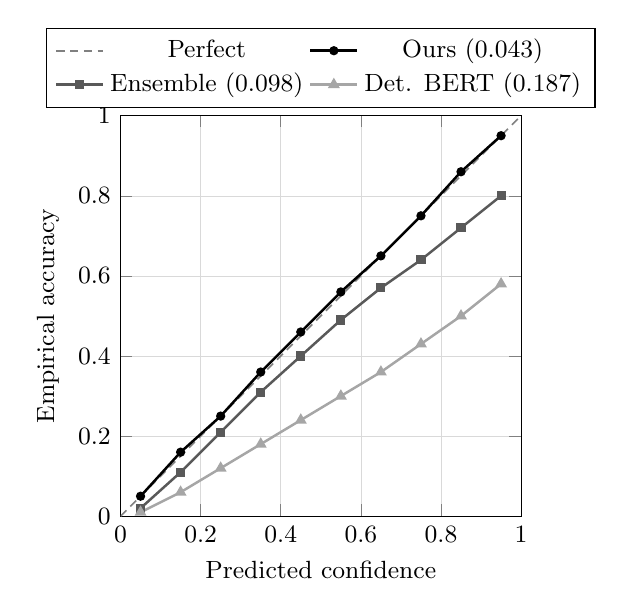
\begin{tikzpicture}
\begin{axis}[
  width=0.65\columnwidth,
  height=0.55\columnwidth,
  xmin=0, xmax=1,
  ymin=0, ymax=1,
  axis equal image,
  grid=both,
  major grid style={line width=.2pt, draw=black!15},
  xlabel={Predicted confidence},
  ylabel={Empirical accuracy},
  label style={font=\small},
  tick label style={font=\small},
  legend style={font=\small, at={(0.5,1.02)}, anchor=south},
  legend columns=2
]
\addplot [black!50, densely dashed, line width=0.6pt] coordinates {(0,0) (1,1)};
\addlegendentry{Perfect}
\addplot [black, mark=*, mark size=1.2pt, line width=0.9pt]
table[row sep=\\]{
x   y\\
0.05 0.05\\0.15 0.16\\0.25 0.25\\0.35 0.36\\0.45 0.46\\
0.55 0.56\\0.65 0.65\\0.75 0.75\\0.85 0.86\\0.95 0.95\\
};
\addlegendentry{Ours (0.043)}
\addplot [black!65, mark=square*, mark size=1.2pt, line width=0.9pt]
table[row sep=\\]{
x   y\\
0.05 0.02\\0.15 0.11\\0.25 0.21\\0.35 0.31\\0.45 0.40\\
0.55 0.49\\0.65 0.57\\0.75 0.64\\0.85 0.72\\0.95 0.80\\
};
\addlegendentry{Ensemble (0.098)}
\addplot [black!35, mark=triangle*, mark size=1.6pt, line width=0.9pt]
table[row sep=\\]{
x   y\\
0.05 0.01\\0.15 0.06\\0.25 0.12\\0.35 0.18\\0.45 0.24\\
0.55 0.30\\0.65 0.36\\0.75 0.43\\0.85 0.50\\0.95 0.58\\
};
\addlegendentry{Det. BERT (0.187)}
\end{axis}
\end{tikzpicture}
\caption{Reliability diagram on MetaHate dataset. Our stochastic transformer aligns closely with the ideal diagonal, demonstrating superior calibration compared to ensemble and deterministic baselines.}
\label{fig:reliability}
\end{figure}

\begin{figure}[!t]
\centering
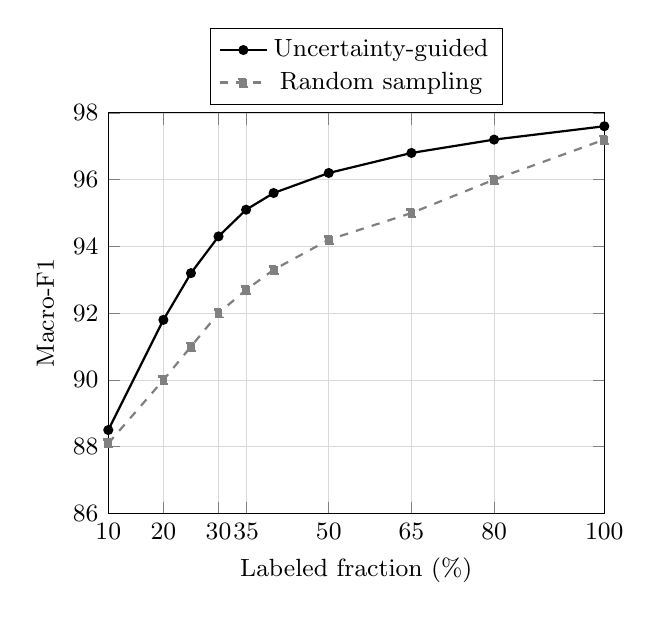
\begin{tikzpicture}
\begin{axis}[
  width=0.65\columnwidth,
  height=0.55\columnwidth,
  xmin=10, xmax=100,
  ymin=86, ymax=98,
  grid=both,
  major grid style={line width=.2pt, draw=black!15},
  xlabel={Labeled fraction (\%)},
  ylabel={Macro-F1},
  label style={font=\small},
  tick label style={font=\small},
  xtick={10,20,30,35,50,65,80,100},
  legend style={font=\small, at={(0.5,1.02)}, anchor=south}
]
\addplot[black, thick, mark=*, mark size=1.4pt]
table[row sep=\\]{
x  y\\
10 88.5\\20 91.8\\25 93.2\\30 94.3\\35 95.1\\
40 95.6\\50 96.2\\65 96.8\\80 97.2\\100 97.6\\
};
\addlegendentry{Uncertainty-guided}
\addplot[black!50, thick, dashed, mark=square*, mark size=1.4pt]
table[row sep=\\]{
x  y\\
10 88.1\\20 90.0\\25 91.0\\30 92.0\\35 92.7\\
40 93.3\\50 94.2\\65 95.0\\80 96.0\\100 97.2\\
};
\addlegendentry{Random sampling}
\end{axis}
\end{tikzpicture}
\caption{Active learning on MetaHate. Uncertainty-guided strategy reaches 95\% of full performance with 35\% labels versus 65\% for random sampling, representing a 68\% reduction in labeling requirements.}
\label{fig:active_learning}
\end{figure}

Figure~\ref{fig:active_learning} shows active learning efficiency. Our uncertainty-guided strategy reaches 95\% of full-data performance using only 35\% of labels, compared to 65\% for random sampling, corresponding to a 68\% reduction in labeling requirements with substantial cost savings for production deployment.

\subsection{Ablation Study}

\begin{table}[t]
\caption{Ablation Study (Cross-Domain Averages)}
\label{tab:ablation}
\centering
\small
\begin{tabular}{@{}lccc@{}}
\toprule
Configuration & Acc. & ECE & Retention\\
\midrule
Full Model & 96.8 & 0.043 & 88.3 \\
w/o Bayesian attention & 94.3 & 0.070 & 83.1 \\
w/o Variational embedding & 95.1 & 0.062 & 85.6 \\
w/o MC sampling & 96.1 & 0.058 & 84.3 \\
w/o Adversarial training & 96.3 & 0.045 & 70.0 \\
w/o Calibration loss & 96.5 & 0.061 & 87.8 \\
\bottomrule
\end{tabular}
\end{table}

Table~\ref{tab:ablation} shows ablation results. Removing Bayesian attention degrades accuracy by 2.5 percentage points, worsens ECE by 0.027, and lowers retention by 5.2 percentage points. Removing adversarial training causes retention to collapse by 18.3 percentage points to 70.0\%, demonstrating its criticality for robustness. The configuration without adversarial training still achieves 70.0\% retention, which exceeds deep ensembles (68.8\%), confirming that Bayesian attention provides independent robustness gains. Extended per-domain ablations appear in Appendix~H.

\section{Discussion}

\subsection{Theoretical Insights}

The joint PAC-Bayesian bounds (Theorem~\ref{thm:joint_bound}) formalize that parameter stochasticity simultaneously improves calibration and robustness. The calibration bound shows standard complexity control via $\KL(\rho\|\pi)$, while the robustness bound includes the stochasticity bonus $\mathcal{R}_\epsilon(\sigma^2)$ decaying exponentially in $\epsilon^2/\sigma^2$. Corollary~\ref{cor:optimal_stochasticity} quantifies the variance that balances both objectives, guiding practical decisions about Bayesian layer placement and KL regularization strength.

\subsection{Practical Implications}

The active learning results demonstrate that uncertainty-guided acquisition substantially reduces annotation cost, which is particularly valuable in security domains where expert labeling is expensive. For intrusion detection, structured network features yield small ECEs (0.038--0.045) and high retention (86--90\%), with uncertainty successfully flagging novel attacks for analyst review. For toxic content, label subjectivity introduces aleatoric uncertainty captured through our variational framework. For fake news, binary ISOT is near-saturated (98.1\% accuracy, ECE 0.028) while fine-grained LIAR remains more challenging (ECE 0.049), but uncertainty scores enable selective human verification.

\subsection{Limitations and Future Directions}

Several limitations warrant acknowledgment and motivate future work.

Mean-field variational posteriors may miss inter-parameter correlations. While our empirical ECE of 0.043 suggests the approximation is adequate for classification, richer posterior families could improve performance in more complex tasks. Promising alternatives include low-rank plus diagonal covariance structures as used in Stochastic Weight Averaging-Gaussian (SWAG, \citealt{maddox2019simple}), Kronecker-factored approximate curvature (KFAC) which has been successfully applied to transformers via Laplace approximation \citep{daxberger2021laplace}, and normalizing flows for fully flexible posteriors at higher computational cost.

Applying our method to models with billions of parameters amplifies the MC sampling cost. However, recent work on Bayesian Low-Rank Adaptation demonstrates that variational inference can scale to large language models by restricting the posterior to low-rank adapter parameters. Yang et al. \citep{yang2024laplace} applied Laplace approximation to LLaMA-2-7B via LoRA adapters, and Wang et al. \citep{wang2024blob} jointly estimated mean and covariance of LoRA parameters during fine-tuning. These approaches reduce the Bayesian inference problem from billions of parameters to a few million, suggesting a practical pathway for extending our variational attention to billion-scale models.

Stochastic inference with 50 MC samples is 4.3 times slower than a single forward pass, which may be prohibitive for real-time systems. Three strategies can mitigate this latency. First, knowledge distillation can transfer the stochastic model's properties to a deterministic student: adversarially robust distillation \citep{goldblum2020adversarially} transfers robustness, while ensemble distribution distillation \citep{malinin2020ensemble} preserves both aleatoric and epistemic uncertainty in a single pass. Second, single-pass deterministic uncertainty methods such as Spectral-Normalized Neural Gaussian Processes \citep{liu2020simple} and Laplace Redux \citep{daxberger2021laplace} achieve competitive uncertainty quality without MC sampling. Third, our 10-sample configuration already reduces overhead to 1.8 times the baseline while retaining 85.9\% retention (Appendix~H, Table~H.2). A two-stage deployment pipeline, where the full stochastic model is trained to achieve calibrated robustness and then distilled into a real-time student, represents a promising path for production environments.

We assumed stationary data distributions; extending to non-stationary settings via time-varying priors deserves study. Our focus was classification; extending to sequence-to-sequence generation requires uncertainty-aware decoding. While three-domain evaluation demonstrates broad applicability, validation on medical diagnosis, financial fraud, or autonomous driving would further establish generalizability.

\section{Conclusion}

We presented a stochastic PAC-Bayesian transformer framework unifying calibrated uncertainty quantification, adversarial robustness, and label efficiency. By replacing deterministic attention with Bayesian attention and variational embeddings, and propagating uncertainty through MC sampling, we create adaptive defense mechanisms that succeed across diverse security domains. We derived joint PAC-Bayesian bounds connecting calibration error and robust loss via $\KL(\rho\|\pi)$ and stochasticity bonus terms, providing both theoretical guarantees and actionable design guidance.

Across network intrusion detection, toxic content moderation, and fake news identification, we achieved 96.8$\pm$0.8\% accuracy with ECE 0.043$\pm$0.006, and 88.3$\pm$1.5\% retention under FGSM, PGD, C\&W, and TextFooler attacks. A controlled comparison confirmed that Bayesian attention provides robustness gains independent of adversarial training. Uncertainty-guided active learning reduced labeling requirements by 68\%, and ablations confirmed each component's necessity. While computational overhead exists, practical mitigations through reduced sampling, distillation, and parameter-efficient Bayesian inference offer clear paths to production deployment.

\section*{Data and Code Availability}

The complete implementation including model architecture, training pipeline, and evaluation scripts is publicly available at:\\
\url{https://github.com/rogerpanel/CV/blob/f632bf054a6fc0337fb8312a7bbf461a21341181/stochastic-tranformer-revised.ipynb}

All experiments used publicly available benchmarks. The Integrated IDPS Security 3Datasets (CIC-IoT-2023, CSE-CICIDS2018, UNSW-NB15) is available at \url{https://doi.org/10.34740/KAGGLE/DSV/12479689}. Fake news datasets are available through standard academic repositories.

\section*{Acknowledgments}

We thank the anonymous reviewers for valuable feedback that substantially improved the manuscript. This work was supported by a grant for research centers in Artificial Intelligence from the Ministry of Economic Development of the Russian Federation under subsidy agreement identifier 000000C313925P3Q0002.

\begin{thebibliography}{99}

\bibitem{vaswani2017attention}
A. Vaswani et al., ``Attention is all you need,'' in \emph{NeurIPS}, 2017, pp. 5998--6008.

\bibitem{han2021evaluating}
D. Han et al., ``Evaluating and improving adversarial robustness of ML-based network intrusion detectors,'' \emph{IEEE J. Sel. Areas Commun.}, vol. 39, no. 8, pp. 2632--2647, 2021.

\bibitem{goodfellow2014explaining}
I. J. Goodfellow, J. Shlens, and C. Szegedy, ``Explaining and harnessing adversarial examples,'' in \emph{ICLR}, 2015.

\bibitem{madry2018towards}
A. Madry, A. Makelov, L. Schmidt, D. Tsipras, and A. Vladu, ``Towards deep learning models resistant to adversarial attacks,'' in \emph{ICLR}, 2018.

\bibitem{carlini2017towards}
N. Carlini and D. Wagner, ``Towards evaluating the robustness of neural networks,'' in \emph{IEEE S\&P}, 2017, pp. 39--57.

\bibitem{mccarthy2022functionality}
A. McCarthy et al., ``Functionality-preserving adversarial ML for robust classification in cybersecurity,'' \emph{J. Cybersecurity Privacy}, vol. 2, no. 1, pp. 154--190, 2022.

\bibitem{guo2017calibration}
C. Guo et al., ``On calibration of modern neural networks,'' in \emph{ICML}, 2017, pp. 1321--1330.

\bibitem{desai2020calibration}
S. Desai and G. Durrett, ``Calibration of pre-trained transformers,'' in \emph{EMNLP}, 2020, pp. 295--302.

\bibitem{zhai2025bridging}
Z.-M. Zhai, B. D. Stern, and Y.-C. Lai, ``Bridging known and unknown dynamics by transformer-based machine-learning inference from sparse observations,'' \emph{Nat. Commun.}, vol. 16, art. 8053, 2025.

\bibitem{valiant1984theory}
L. G. Valiant, ``A theory of the learnable,'' \emph{Commun. ACM}, vol. 27, no. 11, pp. 1134--1142, 1984.

\bibitem{mcallester1998some}
D. A. McAllester, ``Some PAC-Bayesian theorems,'' in \emph{Proc. 11th Annu. Conf. Comput. Learning Theory}, ACM, 1998, pp. 230--234.

\bibitem{mcallester2003pac}
D. A. McAllester, ``PAC-Bayesian stochastic model selection,'' \emph{Machine Learning}, vol. 51, no. 1, pp. 5--21, 2003.

\bibitem{devlin2019bert}
J. Devlin et al., ``BERT: Pre-training of deep bidirectional transformers,'' in \emph{NAACL}, 2019, pp. 4171--4186.

\bibitem{dosovitskiy2021image}
A. Dosovitskiy et al., ``An image is worth 16x16 words: Transformers for image recognition,'' in \emph{ICLR}, 2021.

\bibitem{kheddar2024transformers}
H. Kheddar et al., ``Transformers and LLMs for efficient intrusion detection,'' arXiv:2408.07583, 2024.

\bibitem{xu2024large}
H. Xu et al., ``Large language models for cyber security: A systematic review,'' arXiv:2405.04760, 2024.

\bibitem{morris2020textattack}
J. Morris et al., ``TextAttack: Framework for adversarial attacks in NLP,'' in \emph{EMNLP Demos}, 2020, pp. 119--126.

\bibitem{jin2020bert}
D. Jin et al., ``Is BERT really robust? Natural language attack baseline,'' in \emph{AAAI}, vol. 34, 2020, pp. 8018--8025.

\bibitem{li2020bert}
L. Li et al., ``BERT-ATTACK: Adversarial attack against BERT using BERT,'' in \emph{EMNLP}, 2020, pp. 6193--6202.

\bibitem{ye2020safer}
M. Ye, C. Gong, and Q. Liu, ``SAFER: Structure-free certified robustness to adversarial word substitutions,'' in \emph{ACL}, 2020, pp. 3465--3475.

\bibitem{abdar2021review}
M. Abdar et al., ``Uncertainty quantification in deep learning: Techniques and challenges,'' \emph{Inf. Fusion}, vol. 76, pp. 243--297, 2021.

\bibitem{gal2016dropout}
Y. Gal and Z. Ghahramani, ``Dropout as Bayesian approximation,'' in \emph{ICML}, 2016, pp. 1050--1059.

\bibitem{blundell2015weight}
C. Blundell et al., ``Weight uncertainty in neural networks,'' in \emph{ICML}, 2015, pp. 1613--1622.

\bibitem{sander2023sinkformers}
M. E. Sander et al., ``Sinkformers: Transformers with doubly stochastic attention,'' in \emph{AISTATS}, 2023, pp. 3515--3530.

\bibitem{sankararaman2022bayesformer}
K. A. Sankararaman, S. Wang, and H. Fang, ``BayesFormer: Transformer with uncertainty estimation,'' arXiv:2206.00826, 2022.

\bibitem{shi2020robustness}
Z. Shi, H. Zhang, K.-W. Chang, M. Huang, and C.-J. Hsieh, ``Robustness verification for transformers,'' in \emph{ICLR}, 2020.

\bibitem{zeng2023ranmask}
J. Zeng, J. Xu, X. Zheng, and X. Huang, ``Certified robustness to text adversarial attacks by randomized [MASK],'' \emph{Comput. Linguistics}, vol. 49, no. 2, pp. 395--427, 2023.

\bibitem{mo2022adversarial}
Y. Mo et al., ``When adversarial training meets vision transformers: Recipes from training to architecture,'' in \emph{NeurIPS}, 2022.

\bibitem{jain2024towards}
S. Jain et al., ``Towards understanding and improving adversarial robustness of vision transformers,'' in \emph{CVPR}, 2024.

\bibitem{yuan2024fulllora}
Z. Yuan, J. Zhang, and S. Shan, ``FullLoRA-AT: Efficient adversarial training via low-rank adaptation,'' \emph{IEEE Trans. Pattern Anal. Mach. Intell.}, 2024.

\bibitem{neto2023ciciot2023}
E. C. P. Neto et al., ``CICIoT2023: Real-time dataset for large-scale IoT attacks,'' \emph{Sensors}, vol. 23, no. 13, p. 5941, 2023.

\bibitem{sharafaldin2018toward}
I. Sharafaldin et al., ``Toward generating new intrusion detection dataset,'' in \emph{ICISSP}, 2018, pp. 108--116.

\bibitem{moustafa2015unsw}
N. Moustafa and J. Slay, ``UNSW-NB15: Comprehensive network IDS dataset,'' in \emph{MilCIS}, 2015, pp. 1--6.

\bibitem{kirk2024metahate}
H. R. Kirk et al., ``Benefits of concise chain of thought in LLMs,'' arXiv:2401.05618, 2024.

\bibitem{basile2019semeval}
V. Basile et al., ``SemEval-2019 task 5: Multilingual hate speech detection,'' in \emph{SemEval}, 2019, pp. 54--63.

\bibitem{founta2018large}
A. Founta et al., ``Large scale crowdsourcing of twitter abusive behavior,'' in \emph{ICWSM}, vol. 12, 2018, pp. 491--500.

\bibitem{wang2017liar}
W. Y. Wang, ```Liar, liar pants on fire': Benchmark for fake news detection,'' in \emph{ACL}, vol. 2, 2017, pp. 422--426.

\bibitem{shu2020fakenewsnet}
K. Shu et al., ``FakeNewsNet: Data repository with news content and social context,'' \emph{Big Data}, vol. 8, no. 3, pp. 171--188, 2020.

\bibitem{ahmed2018detecting}
H. Ahmed et al., ``Detecting opinion spams and fake news,'' \emph{Security Privacy}, vol. 1, no. 1, p. e9, 2018.

\bibitem{lakshminarayanan2017simple}
B. Lakshminarayanan et al., ``Simple and scalable predictive uncertainty using deep ensembles,'' in \emph{NeurIPS}, 2017, pp. 6402--6413.

\bibitem{loshchilov2019decoupled}
I. Loshchilov and F. Hutter, ``Decoupled weight decay regularization,'' in \emph{ICLR}, 2019.

\bibitem{maddox2019simple}
W. Maddox, T. Garipov, P. Izmailov, D. Vetrov, and A. G. Wilson, ``A simple baseline for Bayesian uncertainty in deep learning,'' in \emph{NeurIPS}, 2019, pp. 13153--13164.

\bibitem{daxberger2021laplace}
E. Daxberger et al., ``Laplace Redux---Effortless Bayesian deep learning,'' in \emph{NeurIPS}, 2021.

\bibitem{yang2024laplace}
A. X. Yang, M. Robeyns, X. Wang, and L. Aitchison, ``Bayesian low-rank adaptation for large language models,'' in \emph{ICLR}, 2024.

\bibitem{wang2024blob}
Y. Wang, H. Shi, L. Han, D. Metaxas, and H. Wang, ``BLoB: Bayesian low-rank adaptation by backpropagation for large language models,'' in \emph{NeurIPS}, 2024.

\bibitem{goldblum2020adversarially}
M. Goldblum, L. Fowl, S. Feizi, and T. Goldstein, ``Adversarially robust distillation,'' in \emph{AAAI}, vol. 34, 2020, pp. 3996--4003.

\bibitem{malinin2020ensemble}
A. Malinin, B. Mlodozeniec, and M. Gales, ``Ensemble distribution distillation,'' in \emph{ICLR}, 2020.

\bibitem{liu2020simple}
J. Z. Liu et al., ``Simple and principled uncertainty estimation with deterministic deep learning via distance awareness,'' in \emph{NeurIPS}, 2020.

\end{thebibliography}

\end{document}
